\chapter{Gesichtserkennung}
% 2D BV, Machine Learning -> viola-jones-methode (haar-wavelets)
% opencv Funktionsweise (Dokumentation)
% frontal, profile
% probleme, Ergebnisse
Die Aufgabenstellung beinhaltet, in den extrahierten Fotos Gesichter zu erkennen. Hier muss die Gesichtserkennung (in der Fachliteratur "Face Detection") von der Wiedererkennung von bereits identifizierten Gesichtern (in der Fachliteratur "Face Recognition") unterschieden werden. In der vorliegenden Arbeit geht es ausschließlich darum, die Position von Gesichtern in den eingescannten Fotos zu erkennen und nicht, bereits erkannte Gesichter wiederzuerkennen oder zuzuordnen \footnote{Aufgrund der geringen Datenmenge und der schlechten Qualität der alten Fotos ist es nicht möglich, Gesichter wiederzuerkennen.}.\\
In der klassischen Bildverarbeitung wurden lange einfache 2D-Verfahren verwendet, um Gesichter in Bildern zu erkennen (\cite{Kees2012}, \cite{Wachter2001}). Beim Template Matching werden beispielsweise Vorlagen (von Teilen) von Gesichtern erzeugt um diese dann im Anwendungsfall mit den Zielbildern zu vergleichen. Dieses Verfahren ist nicht sehr robust, besonders bei sich verändernden Lichtverhältnissen, aber gleichzeitig extrem rechenaufwändig. \\
Eine einfachere Methode der Gesichtserkennung in der klassischen Bildverarbeitung ist die Nutzung von geometrischen Merkmalen in den Gesichtern. Hierbei werden beispielsweise Grauwerte in einem bestimmten Bereich des Bildes aufsummiert oder Gradientenoperatoren zur horizontalen und vertikalen Kantenerkennung angewandt. So kann die Ausrichtung, die relative Lage und ähnliche Merkmale der Nase, der Augen und des Munden identifiziert und zusammen als Gesicht klassifiziert werden. \\
Doch auch diese Methode ist rechen- und zeitintensiv. Deswegen wird häufig eher auf komplexere Methoden zur Gesichtserkennung gesetzt, wie beispielsweise das Elastic Bunch Graph Matching, das eine robuste Waveletanalyse nutzt (\cite{Wiskott1999}) oder die auf der Hauptkomponentenanalyse basierende Eigenfaces-Methode (\cite{doi:10.1162/jocn.1991.3.1.71}). Weiterentwicklungen dieser beiden Methoden werden heute noch eingesetzt, obwohl die Ansätze schon vergleichsweise alt sind. \\
Im Folgenden wird ein populärer Ansatz vorgestellt, der in den vorliegenden Arbeit verwendet wurde. 

\section{Cascade Classifier}
Die OpenCV Programmbibliothek beinhaltet vorimplementierte Funktionen zur Gesichtserkennung. Sie basiert auf einem 2001 entwickelten Ansatz zur Objekterkennung in Bildern (\cite{Viola2001}, \cite{Lienhart2002}). Es ist ein trainierter Classifier, der einfache geometrische Merkmale im Bild erkennt und auf deren Basis die gewünschten Objekte erkennen kann (\cite{OpenCV}).\\
Die Methode nutzt sogenannte Haar-ähnliche Features, mit denen grundlegende Strukturen (Helligkeitsunterschiede) im Bild erkannt werden. Im Bild \ref{fig:haarfeatures} werden alle Features aufgelistet, die der Classifier nutzen kann. Für die Gesichtserkennung werden in der Praxis aber nicht so viele genutzt, sondern nur einige wenige. Mit diesen können allgemeine Eigenschaften von menschlichen Gesichtern repräsentiert werden. So ist zum Beispiel die Nase heller als die Bereiche um die Augen, das entspricht dem Feature 2(a) in Bild \ref{fig:haarfeatures}.\\
\begin{figure}
	\centering
	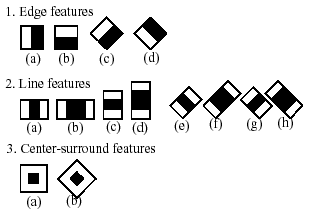
\includegraphics[width=0.5\linewidth]{images/haarfeatures.png}
	\caption{Alle vom Cascade Classifier Algorithmus genutzten Haar-ähnlichen Features zur Objekterkennung. Zur Gesichtserkennung werden nur fünf Features genutzt: 1(a), 1(b), 2(a), 2(c) und eine Kombination aus zwei 1(a) Features, die zusammen ein schachbrettartiges Muster ergeben.}
	\label{fig:haarfeatures}
\end{figure}
Nachdem die zu nutzenden Features ausgewählt wurden, wird ein Integralbild erzeugt, das in der Lage ist, die Features in konstanter Zeit auszuwerten. Dadruch wird eine relativ geringe Laufzeit erzielt.\\
In der Trainingsphase wird der Classifier mit Positiv- und Negativbeispielen von dem zu erkennenden Objekt trainiert, in diesem Fall mit Gesichtern \footnote{In der OpenCV Bibliothek ist sowohl ein Trainer als auch ein Detector enthalten. Der Detector ist vortrainiert kann direkt zur Gesichtserkennung verwendet werden. Wenn man genug Daten zur Verfügung hat, kann man aber auch einen selbst trainieren.}. Dieser Vorgang wird mit verschiedenen Arten des AdaBoostings beschleunigt und verbessert. Dadurch werden die besten Features für die Klassifizierung identifiziert. \\
Danach wird der Classifier in mehreren Stufen auf die Bilder angewandt ("cascade"), in denen das Objekt identifiziert werden soll. Jeder Classifier funktioniert dabei wie ein Filter, der die negativen Regionen aus dem Bild herausfiltert. Die verbleibenden Bereiche werden Stück für Stück durch immer komplexere Classifier gegeben, bis sie entweder aussortiert werden oder das Objekt (ein Gesicht) identifiziert wurde. Somit hat der Cascade Classifier die Struktur eines Entscheidungsbaumes und Rechenzeit wird gespart. Die Methode ist so robust, dass das Objekt in verschiedenen Größen in dem Bild erkennen kann, unabhängig von der Größe der Bilder, mit der der Classifier trainiert wurde.\\
Wenn die OpenCV Methode \texttt{detectMultiScale} ein Gesicht im Input-Bild erkennt, gibt es die Position in x- und y-Koordinaten und dessen Abmessungen (Höhe, Breite) zurück. In dem vorliegenden Programm werden zwei verschiedene Classifier auf die Bilder angewandt: einmal frontale Gesichter und einmal Gesichter im Profil. Die Rückgabewerte der Funktionen werden dafür genutzt, die Gesichter auszuschneiden und Dopplungen zu erkennen.
% nutzung in der praxis: https://docs.opencv.org/3.4/d7/d8b/tutorial_py_face_detection.html